\section{Dealing with data}
Given that \pkg{StochBB} is able to provide a good approximation of the PDF of some (response) random variable, it is also able to fit a system of dependent random variables to data. For this, the \pkg{StochBB} API provides two function. One is the \code{kolmogorov} function which returns the Kolmogorov-Smirnov statistic \cite[e.g.,][]{Marsaglia2003}, the other function is the \code{logLikelihood} function. Both take the random variable, the   number of bins and some data vector as arguments. Both function then uses an approximation of the PDF (for the log likelihood) or CDF (KS) evaluated on a regular grid spanning the data range for computing the corresponding value.

These functions can then be used to fit a network of random variables to some given observations. For example, consider the network of random variables introduced above, describing the cognitive process under the \emph{experimental condition}. One may try to re-estimate the $\theta=120$ parameter of the stage S2. First, a relatively large sample is drawn ($N=10,000$). Then one may implement a cost function of that parameter, that is the negative of the log likelihood given the samples and finally fit that mode the the data by minimizing the cost function using a numerical optimization algorithm.

An example R code could be
\begin{lstlisting}[language=R, basicstyle=\footnotesize]
library(stochbb)

# The "stages"
d  <- 500
V  <- gamma(5,30)
S1 <- gamma(10,50)
S2 <- gamma(1,120)
M  <- gamma(1,150) 

# Response under "experimental condition"
Re <- V %+% minimum(S1, S2 %+% d) %+% M

# Sample Re
Nsam <- 30000;
sam <- new(ExactSampler, c(Re))
res <- array(0, c(Nsam,1))
sam$sample(res)

costFunc <- function(theta) {
  S2 <- gamma(1,theta[1]);
  R <- V %+% minimum(S1, affine(S2, 1, d)) %+% M
  return( -logLikelihood(R, 10000, res[,1]) )
}

# Find estimate
opt <- optim(c(100), costFunc, method="L-BFGS-B")
\end{lstlisting}

This code is then able to find the $\theta$ parameter for the S2 stage by means of maximum likelihood. 

\begin{figure}[!ht]
 \centering
 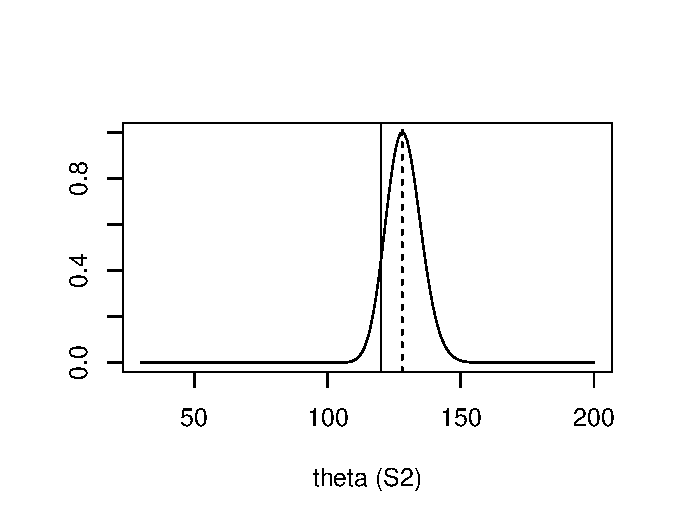
\includegraphics[width=0.49\textwidth]{fig/pod_likelihoodProf.pdf}
 \caption{An example of a likelihood profile for some $\theta$ estimate using 10,000 samples.} \label{fig:llprof}
\end{figure}

Moreover, the \code{logLikelihood} can then also be used to profile the likelihood (see Figure \ref{fig:llprof}) given the data to obtain confidence intervals for the parameter estimate. There the true value of $\theta=120$ is shown as a solid vertical line and the estimate as the dashed vertical line. 